\begin{name}
	{\tenchude}
	{TOÁN 10}
	{LỚP TOÁN THẦY PHÁT}
	{Thời gian: 90 phút - Không kể thời gian phát đề}
\end{name}
\noindent{\bf\fontfamily{qag}\selectfont\color{violet}A. PHẦN TRẮC NGHIỆM}
\Opensolutionfile{ans}[ans/ans-0-GK1-CTST-De8-NH23-24]

\begin{ex}%[PC06-0-GK1-NH23-24--TeamTeXHoa--Lê Quân]%[0T1Y1-3]
	Mệnh đề phủ định của mệnh đề \lq\lq  $\exists x\in \mathbb{N}, x=-x$\rq\rq \, là 
	\choice
	{$\forall x\in \mathbb{N}, x=-x$}
	{$\exists x\in \mathbb{N}, x\ne -x$}
	{$\forall x\in \mathbb{N}, x>-x$}
	{\True $\forall x\in \mathbb{N}, x\ne -x$}
	\loigiai
	{
	Mệnh đề phủ định của mệnh đề \lq\lq  $\exists x\in \mathbb{N}, x=-x$\rq\rq \, là mệnh đề \lq\lq  $\forall x\in \mathbb{N}, x\ne x$\rq\rq.	
	}
\end{ex}

\begin{ex}%[PC06-0-GK1-NH23-24--TeamTeXHoa--Lê Quân]%[0T1Y1-3]
	Mệnh đề $P\colon$ \lq\lq  $\forall x\in \mathbb{R}, 28x^2-9x+2022<0$\rq\rq\, có mệnh đề phủ định là mệnh đề nào trong các mệnh đề sau?
	\choice
	{$\exists x\in \mathbb{R}, 28x^2-9x+2022>0$}
	{$\forall x\in \mathbb{R}, 28x^2-9x+2022>0$}
	{$\forall x\notin \mathbb{R}, 28x^2-9x+2022\ge 0$}
	{\True $\exists x\in \mathbb{R}, 28x^2-9x+2022\ge 0$}
	\loigiai
	{
	Mệnh đề phủ định của mệnh đề $P$ là $\overline{P}$: \lq\lq  $\exists x\in \mathbb{R}, 28x^2-9x+2022\ge 0$\rq\rq.	
	}
\end{ex}

\begin{ex}%[PC06-0-GK1-NH23-24--TeamTeXHoa--Lê Quân]%[0T1Y1-2] 
Trong các mệnh đề sau, mệnh đề nào {\bf sai}?
\choice
{$\forall n\in \mathbb{N}$, $2n$ là số chẵn}
{$\forall x\in \mathbb{R}, x^2\ge 0$}
{$\exists n\in \mathbb{N}, n^2=n$}
{\True $\forall n\in \mathbb{N}, -n^2<0$}
\loigiai{
Xét mệnh đề \lq\lq  $\forall n\in \mathbb{N}, -n^2<0$\rq\rq, thử với $n=0$ ta được $-n^2=0$ nên mệnh đề $\forall n\in \mathbb{N}, -n^2<0$ là mệnh đề sai.
}
\end{ex}

\begin{ex}%[PC06-0-GK1-NH23-24--TeamTeXHoa--Lê Quân]%[0T1Y2-1] 
Hãy liệt kê các phần tử của tập hợp $A$ gồm tất cả các số tự nhiên chia hết cho $7$ và nhỏ hơn $50$.
\choice
{$A=\{ 7; 14; 21; 28; 35; 42; 49  \}$}
{$A=\{ 7; 14; 21; 28; 35; 42 \}$}
{\True $A=\{0; 7; 14; 21; 28; 35; 42; 49  \}$}
{$A=\{  0; 14; 21; 28; 35; 42; 49\}$}
\loigiai{
Các số tự nhiên nhỏ hơn $50$ và chia hết cho $7$ gồm $0; 7; 14; 21; 28; 35; 42; 49$.
}
\end{ex}

\begin{ex}%[PC06-0-GK1-NH23-24--TeamTeXHoa--Lê Quân]%[0T1Y2-1] 
Cho tập hợp $A=\{1; 2; 3; 4; 5\}$. Khẳng định nào sau đây đúng?
\choice
{$A=\{x\in \mathbb{R}|\,0<x<6\}$}
{\True $A=\{x\in \mathbb{N}|\,0<x<6\}$}
{$A=\{x\in \mathbb{Z}|\,x\le 5\}$}
{$A=\{x\in \mathbb{N}|\,x\le 5\}$}
\loigiai{
Ta có $A=\{x\in \mathbb{N}|\,0<x<6\}$.
}
\end{ex}

\begin{ex}%[PC06-0-GK1-NH23-24--TeamTeXHoa--Lê Quân]%[0T1B3-4] 
Cho hai tập hợp $A=[-5; 3)$ và $B=(1; +\infty)$. Khẳng định nào sau đây đúng?
\choice
{\True $A\cap B=(1; 3)$}
{$A\cap B=(1; 3]$}
{$A\cap B=[-5; +\infty)$}
{$A\cap B=[-5; 1]$}
\loigiai{
Ta có $A\cap B=(1; 3)$.
}
\end{ex}

\begin{ex}%[PC06-0-GK1-NH23-24--TeamTeXHoa--Lê Quân]%[0T1Y3-3] 
\immini{Cho hai tập hợp $C$ và $D$ được biểu diễn bằng biểu đồ Ven như hình vẽ. Khẳng định nào sau đây đúng?
\choice
{$C\cap D=\{3; 5; 7; 9\}$}
{$C\cap D=\{7\}$}
{\True $C\cap D=\{3; 5\}$}
{$C\cap D=\{3; 5; 7\}$}
}
{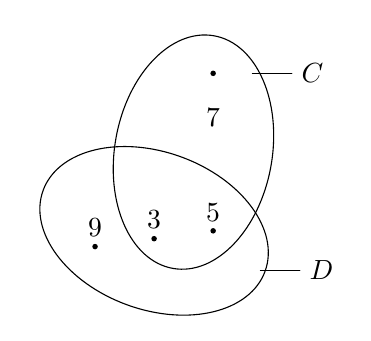
\begin{tikzpicture}[scale=0.5,line join=round, line cap=round, >=stealth]
	\coordinate (A) at (0,-1);
	\coordinate (B) at (-1,-3);
	\draw[rotate=80] (A) ellipse (3cm and 2cm);
\begin{scope}[yshift =2]
		\draw[rotate=-20](B) ellipse (3cm and 2cm);
\end{scope}
	\draw(-1,-3.2) node[above ]{$3$};
	\draw(.5,-3) node[above ]{$5$};
	\draw(.5,-0.6) node[above ]{$7$};
	\draw(-2.5,-3.4) node[above ]{$9$};
	\draw(1.7,-4)  --(2.7, -4)node[right ]{$D$};
	\draw(1.5,1)  --(2.5, 1)node[right ]{$C$};
	\fill[black](-1,-3.2)  circle (2pt);
	\fill[black](.5,-3)  circle (2pt);
	\fill[black](.5,1)   circle (2pt);
		\fill[black](-2.5,-3.4)  circle (2pt);
\end{tikzpicture}}
\loigiai{
Ta có $C\cap D=\{3; 5\}$.
}
\end{ex}

\begin{ex}%[PC06-0-GK1-NH23-24--TeamTeXHoa--Lê Quân]%[0T1B3-3] 
Lớp $10A$ tham gia thi học sinh giỏi cấp trường, trong đó có $25$ học sinh tham gia thi môn Toán, $20$ học sinh tham gia thi môn Văn và có $15$ học sinh tham gia thi cả hai môn Toán và Văn. Hỏi lớp $10A$ có bao nhiêu học sinh tham gia thi ít nhất một trong hai môn Văn và Toán?
\choice
{$35$}
{$40$}
{$45$}
{\True $30$}
\loigiai{
\immini{
Kí hiệu $A$ và $B$ lần lượt là tập hợp các học sinh của lớp $10A$ tham gia thi học sinh giỏi môn Toán và môn Văn.\\
Theo giả thiết ta có $n(A)=25, n(B)=20$ và $n(A\cap B)=15$.\\
$\Rightarrow n(A\cup B)=n(A)+n(B)-n(A\cap B)=25+20-15=30$.\\
Vậy số học sinh tham gia thi ít nhất một trong hai môn là $30$ học sinh
}
{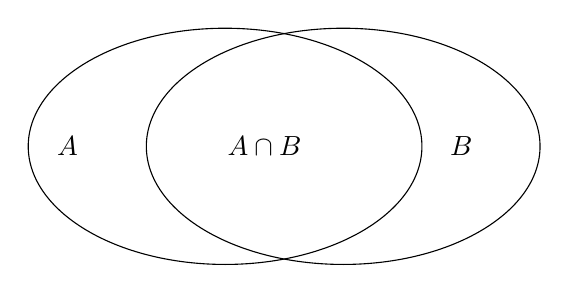
\begin{tikzpicture}[scale=0.5,line join=round, line cap=round, >=stealth]
\draw (0,0) ellipse (5 cm and 3 cm);
\draw (3,0) ellipse (5 cm and 3 cm);
	\draw(1,0) node{$A\cap B$};
	\draw(-4,0) node{$A$};
		\draw(6,0) node{$B$};
\end{tikzpicture}}
}
\end{ex}

\begin{ex}%[PC06-0-GK1-NH23-24--TeamTeXHoa--Lê Quân]%[0T1B3-5] 
Cho hai tập hợp $A=[-3;2]$ và $B=\{x\in \mathbb{R}|\, x<-1\}$. Tìm $A\cap B$.		
\choice
{\True $A\cap B =[-3; -1)$}
{$A\cap B=(-1; 2]$}
{$A\cap B=[-3; 2]$}
{$A\cap B(-\infty; -1)$}
\loigiai{
Ta có $B=(-\infty; -1)$ nên $A\cap B=[-3; -1)$.
}
\end{ex}

\begin{ex}%[PC06-0-GK1-NH23-24--TeamTeXHoa--Lê Quân]%[0T1B3-5] 
Cho tập hợp $A=\{x\in \mathbb{R}|\, -1\le x<3\}$. Tìm $C_{\mathbb{R}}A$.	
\choice
{$C_{\mathbb{R}}A=(-\infty; -1)$}
{$C_{\mathbb{R}}A=(-\infty; -1]\cup (3; +\infty)$}
{\True 	$C_{\mathbb{R}}A=(-\infty; -1)\cup [3; +\infty)$}
{$C_{\mathbb{R}}A=[3; +\infty)$}
\loigiai{
Ta có $A=[-1; 3)$ nên $C_{\mathbb{R}}A =(-\infty; -1)\cup [3; +\infty)$.
}
\end{ex}

\begin{ex}%[PC06-0-GK1-NH23-24--TeamTeXHoa--Lê Quân]%[0T2Y1-2] 
Điểm $O(0; 0)$ thuộc miền nghiệm của bất phương trình nào sau đây?
\choice
{$x+3y+2\le 0$}
{$x+y+2\le 0$}
{$2x+5y-2\geq 0$}
{\True $2x+y+2\ge 0$}
\loigiai{
Dễ thấy tọa độ điểm $O(0; 0)$ thỏa mãn bất phương trình $2x+y+2\ge 0$ nên điểm $O(0; 0)$ thuộc miền nghiệm của bất phương trình $2x+y+2\ge 0$.
}
\end{ex}

\begin{ex}%[PC06-0-GK1-NH23-24--TeamTeXHoa--Lê Quân]%[0T2Y1-2] 
Cặp số nào sau đây {\bf không} là nghiệm của bất phương trình $5x-2(y-1)\le 0$?
\choice
{$(0; 1)$}
{\True $(1; 3)$}
{$(-1; 1)$}
{$(-1; 0)$}
\loigiai{
Dễ thấy cặp số $(1; 3)$ không thỏa mãn bất phương trình $5x-2(y-1)\le 0$.
}
\end{ex}

\begin{ex}%[PC06-0-GK1-NH23-24--TeamTeXHoa--Lê Quân]%[0T2Y1-2] 
Miền nghiệm của bất phương trình $3x+2(y+3)\ge 4(y+1)-y+3$ chứa điểm nào trong các điểm sau?
\choice
{$(3; 0)$}
{\True $(3; 1)$}
{$(2; 1)$}
{$(0; 0)$}
\loigiai{
Ta có $3x+2(y+3)\ge 4(y+1)-y+3\Leftrightarrow -x+3y-1\ge 0.\quad (1)$\\
Dễ thấy cặp số $(2; 1)$ thỏa mãn bất phương trình $(1)$.\\
Vậy miền nghiệm của bất phương trình đã cho chứa điểm $(2; 1)$.
}
\end{ex}

\begin{ex}%[PC06-0-GK1-NH23-24--TeamTeXHoa--Lê Quân]%[0T2Y1-2] 
Miền nghiệm của bất phương trình $5(x+2)-9<2x-2y+7$ {\bf không} chứa điểm nào trong các điểm sau?
\choice
{$(0; 0)$}
{$(2; -1)$}
{$(-2; 1)$}
{\True $(2; 3)$}
\loigiai{
Ta có $5(x+2)-9<2x-2y+7\Leftrightarrow 3x+2y-6<0.\quad (1)$
\\
Dễ thấy cặp số $(2; 3)$ không thỏa mãn bất phương trình $(1)$.\\
Vậy miền nghiệm của bất phương trình đã cho không chứa điểm $(2; 3)$.
}
\end{ex}

\begin{ex}%[PC06-0-GK1-NH23-24--TeamTeXHoa--Lê Quân]%[0T2Y1-2] 
Miền nghiệm của bất phương trình $3x-2y>-6$ là
\choice
	{\begin{tikzpicture}[>=stealth,line join=round,line cap=round,font=\footnotesize,scale=0.4]
			\clip (-2,-2) rectangle (3.5,4.5);
			\draw[->] (-2,0)--(3.5,0) node[below left]{$x$};
			\draw[->] (0,-2)--(0,4.5) node[below right]{$y$};
			\fill[name=O] (0,0) circle (1.2pt) node[below left, fill=white] {$O$}; 
			\draw[color=black, smooth, samples=200, domain= -1:3.5] plot(\x,{-3/2*(\x) + 3}) ;
			\fill[pattern=north east lines, fill opacity=0.5] (-2,5)-- plot[color=black, smooth, samples=100, domain= -1.1:3] (\x,{-3/2*(\x) + 3}) -- (4,-3)--(-2,-3)--cycle;
			\coordinate[label=right:{$3$}] (3y) at (0,3);
			\coordinate[label=above right:{$2$}] (2x) at (2,0);
			\foreach \p in {3y,2x}
			\fill (\p) circle (1.3pt);
	\end{tikzpicture}}
	{
		\begin{tikzpicture}[>=stealth,line join=round,line cap=round,font=\footnotesize,scale=0.4]
			\clip (-3.2,-2) rectangle (3,4.5);
			\draw[->] (-3.5,0)--(2.5,0) node[below left]{$x$};
			\draw[->] (0,-2)--(0,4.5) node[below left]{$y$};
			\fill[name=O] (0,0) circle (1.2pt) node[below left] {$O$}; 
			\draw[color=black, smooth, samples=200, domain= -3:2] plot(\x,{3/2*(\x) + 3}) ;
			\fill[pattern=north east lines, fill opacity=0.5] (-3,-2)-- plot[color=black, smooth, samples=100, domain= -3:2] (\x,{3/2*(\x) + 3}) -- (2.5,4.5)--(2.5,-2)--cycle;
			\coordinate[label=left:{$3$}] (3y) at (0,3);
			\coordinate[label=above left:{$-2$}] (-2x) at (-2,0);
			\foreach \p in {3y,-2x}
			\fill (\p) circle (1.3pt);
	\end{tikzpicture}}
	{\True 
		\begin{tikzpicture}[>=stealth,line join=round,line cap=round,font=\footnotesize,scale=0.4]
			\clip (-3.75,-2) rectangle (2.5,4.5);
			\draw[->] (-3.75,0)--(2,0) node[below left]{$x$};
			\draw[->] (0,-2)--(0,4.5) node[below left]{$y$};
			\fill[name=O] (0,0) circle (1.2pt) node[below left] {$O$}; 
			\draw[color=black, smooth, samples=200, domain= -3.75:2] plot(\x,{3/2*(\x) + 3}) ;
			\fill[pattern=north east lines, fill opacity=0.5] (-3.75,-2)-- plot[color=black, smooth, samples=100, domain= -3.75:2] (\x,{3/2*(\x) + 3}) -- (-3.75,4.5)--(-3.75,-2)--cycle;
			\coordinate[label=right:{$3$}] (3y) at (0,3);
			\coordinate[label=below:{$-2$}] (-2x) at (-2,0);
			\foreach \p in {3y,-2x}
			\fill (\p) circle (1.3pt);
	\end{tikzpicture}}
	{\begin{tikzpicture}[>=stealth,line join=round,line cap=round,font=\footnotesize,scale=0.4]
			\clip (-3,2) rectangle (3,-4.5);
			\draw[->] (-3.5,0)--(2.5,0) node[below left]{$x$};
			\draw[->] (0,-4.5)--(0,2) node[below left]{$y$};
			\fill[name=O] (0,0) circle (1.2pt) node[below left] {$O$}; 
			\draw[color=black, smooth, samples=200, domain= -3:2] plot(\x,{-3/2*(\x) - 3});
			\fill[pattern=north east lines, fill opacity=0.5] (-3,2)-- plot[color=black, smooth, samples=100, domain= -3:2] (\x,{-3/2*(\x) - 3}) -- (2,-4.5)--(-3,-4.5)--cycle;
			\coordinate[label=right:{$-3$}] (-3y) at (0,-3);
			\coordinate[label=above:{$-2$}] (-2x) at (-2,0);
			\foreach \p in {-3y,-2x}
			\fill (\p) circle (1.3pt);
	\end{tikzpicture}}
\loigiai{
		\immini{
			Xét đường thẳng $d\colon 3x-2y=-6$.\\
			Ta có đường thẳng này đi qua hai điểm $(-2;0)$ và $(0;3)$.\\
			Thay tọa độ điểm $O(0;0)$ vào, ta có $3x-2y=0>-6$.\\
			Vậy miền nghiệm của bất phương trình đã cho là nửa mặt phẳng có bờ là đường thẳng $d\colon 3x-2y=-6$, không tính bờ $d$ và không chứa gốc tọa độ $O(0;0)$ (miền không bị gạch).}
		{
			\begin{tikzpicture}[>=stealth,line join=round,line cap=round,font=\footnotesize,scale=0.6]
				\clip (-3,-2) rectangle (3,4.5);
				\draw[->] (-3.5,0)--(2.5,0) node[below left]{$x$};
				\draw[->] (0,-2)--(0,4.5) node[below left]{$y$};
				\fill[name=O] (0,0) circle (1.2pt) node[below left] {$O$}; 
				\draw[color=black, smooth, samples=200, domain= -3:2] plot(\x,{3/2*(\x) + 3}) node[left]{$ $};
				\fill[pattern=north east lines, fill opacity=0.5] (-3,-2)-- plot[color=black, smooth, samples=100, domain= -3:2] (\x,{3/2*(\x) + 3}) -- (2.5,4.5)--(2.5,-2)--cycle;
				\coordinate[label=left:{$3$}] (3y) at (0,3);
				\coordinate[label=above left:{$-2$}] (-2x) at (-2,0);
				\foreach \p in {3y,-2x}
				\fill (\p) circle (1.3pt);
			\end{tikzpicture}
		}
	}	
\end{ex}

\begin{ex}%[PC06-0-GK1-NH23-24--TeamTeXHoa--Lê Quân]%[0T2Y2-3] 
Điểm $O(0; 0)$ thuộc miền nghiệm của hệ bất phương trình nào sau đây?
\choice
{$\heva{&x+3y-6>0	\\&2x+y+4>0}$}
{$\heva{&x+3y-6>0	\\&2x+y+4<0}$}
{\True $\heva{&x+3y-6<0	\\&2x+y+4>0}$}
{$\heva{&x+3y-6<0	\\&2x+y+4<0}$}
\loigiai{
Thay tọa độ điểm $O(0; 0)$ vào từng đáp án ta thấy cặp số $(0;0)$ thỏa mãn hệ $\heva{&x+3y-6<0	\\&2x+y+4>0.}$
}
\end{ex}

\begin{ex}%[PC06-0-GK1-NH23-24--TeamTeXHoa--Lê Quân]%[0T2Y2-3] 
Cặp số nào trong các cặp số sau {\bf không} phải là nghiệm của hệ bất phương trình $\heva{&x+y-2\le 0	\\&2x-3y+2>0}$?
\choice
{$(0; 0)$}
{$(1; 1)$}
{\True $(-1; 1)$}
{$(-1; -1)$}
\loigiai{
Dễ thấy, cặp số $(-1; 1)$ không thỏa mãn hệ bất phương trình đã cho.
}
\end{ex}
\begin{ex}%[PC06-0-GK1-NH23-24--TeamTeXHoa--Lê Quân]%[0T2Y2-3] 
Điểm nào sau đây thuộc miền nghiệm của hệ bất phương trình $\heva{&2x-5y-1>0	\\&2x+y+5>0\\&x+y+1<0}$?
\choice
{$(0; 0)$}
{$(1; 0)$}
{\True $(0; -2)$}
{$(0; 2)$}
\loigiai{
Dễ thấy cặp số $(0; -2)$ thỏa mãn hệ bất phương trình đã cho.
}
\end{ex}

\begin{ex}%[PC06-0-GK1-NH23-24--TeamTeXHoa--Lê Quân]%[0T2B2-3] 
\immini{ Phần không gạch chéo trong hình bên là biểu diễn miền nghiệm của hệ bất phương trình nào trong các hệ bất phương trình sau?
\choice
{\True $\heva{&y>0	\\&3x+2y<6}$}
{$\heva{&y>0	\\&3x+2y<-6}$}
{$\heva{&x>0	\\&3x+2y<6}$}
{$\heva{&x>0	\\&3x+2y>-6}$}}
{\begin{tikzpicture}[>=stealth,line join=round,line cap=round,font=\footnotesize,scale=0.4]
	\clip (-2,-2) rectangle (3.5,4.5);
	\draw[->] (-2,0)--(3.5,0) node[below left]{$x$};
	\draw[->] (0,-2)--(0,4.5) node[below right]{$y$};
	\fill[name=O] (0,0) circle (1.2pt) node[above left] {$O$}; 
	\draw[color=black, smooth, samples=200, domain= -1:3.5] plot(\x,{-3/2*(\x) + 3}) ;
	\fill[pattern=north east lines, fill opacity=0.5] (4,-3)-- plot[color=black, smooth, samples=100, domain= -1.1:3] (\x,{-3/2*(\x) + 3}) -- (-1.3,5)--(4,5)--cycle;
		\fill[pattern=north east lines, fill opacity=0.5] (-2,-3)rectangle (4,0) ;
	\coordinate[label=left:{$3$}] (3y) at (0,3);
	\coordinate[label=above left :{$2$}] (2x) at (2,0);
	\foreach \p in {3y,2x}
	\fill (\p) circle (1.3pt);
\end{tikzpicture}}
\loigiai{
Từ hình vẽ ta thấy, điểm $(-1; 1)$ thuộc miền nghiệm của hệ bất phương trình.\\
Bộ số $(1; 1)$ chỉ thỏa mãn hệ  $\heva{&y>0	\\&3x+2y<6.}$\\
Vậy miền nghiệm đã cho là của hệ $\heva{&y>0	\\&3x+2y<6.}$
}
\end{ex}

\begin{ex}%[PC06-0-GK1-NH23-24--TeamTeXHoa--Lê Quân]%[0T2B2-3] 
Cho hệ bất phương trình $\heva{&2x+3y<5	&\quad (1)\\&x+\dfrac{3}{2}y<5&\quad (2)}$. Gọi $S_1, S_2$ lần lượt là tập nghiệm của bất phương trình $(1)$ và $(2)$, $S$ là tập nghiệm của hệ phương trình. Khẳng định nào sau đây đúng?
\choice
{\True $S_1\subset S_2$}
{$S_2\subset S_1$}
{$S_2=S$}
{$S_1\neq S$}
\loigiai{
\immini{
Vẽ hai đường thẳng $d_1\colon 2x+3y-5=0$ và đường thẳng $d_2\colon x+\dfrac{3}{2}y-5=0$.
\\
Ta thấy cặp số $(0; 0)$ là nghiệm của cả hai bất phương trình nên tập nghiệm của hệ bất phương trình là miền không bị gạch như hình bên.\\
Vậy $S_1\subset S_2$.
}
{\begin{tikzpicture}[>=stealth,line join=round,line cap=round,font=\footnotesize,scale=0.4]
	\clip (-4.2,-3) rectangle (7,5.8);
	\draw[->] (-4,0)--(6,0) node[right]{$x$};
	\draw[->] (0,-2)--(0,5) node[above]{$y$};
	\fill[name=O] (0,0) circle (1.2pt) node[above left] {$O$}; 
	\draw[color=black, smooth, samples=200, domain= -4.2:5.1] plot(\x,{-2/3*(\x) + 5/3})node[below right]{$d_1$} ;
	\draw[color=black, smooth, samples=200, domain= -2:5.5] plot(\x,{-2/3*(\x) + 10/3})node[below right]{$d_2$};
	\fill[pattern = horizontal lines, fill opacity=0.5] (5.5,-0.3)-- plot[color=black, smooth, samples=100, domain=  -2:5] (\x,{-2/3*(\x) + 10/3}) -- (-2,4.7)--(5.5,4.7)--cycle;
	\fill[pattern=north east lines, fill opacity=0.5] (5.5,-2)-- plot[color=black, smooth, samples=100, domain=  -4:5] (\x,{-2/3*(\x) + 5/3})-- (-4.5,4.7)--(5,4.7)--cycle;

\end{tikzpicture}}
} 
\end{ex}

\begin{ex}%[PC06-0-GK1-NH23-24--TeamTeXHoa--Lê Quân]%[0T4Y1-3] 
Khẳng định nào sau đây đúng với với mọi góc $\alpha$?
\choice
{$\sin^2 \alpha -\cos^2\alpha =1$}
{$\sin^2\alpha-\cos^2\alpha=-1$}
{$\sin^2\alpha-\cos^2\alpha=0$}
{\True $\sin^2\alpha+\cos^2\alpha=1$}
\loigiai{
Ta có $\sin^2\alpha+\cos^2\alpha=1$, $\forall \alpha \in \mathbb{R}$.
}
\end{ex}

\begin{ex}%[PC06-0-GK1-NH23-24--TeamTeXHoa--Lê Quân]%[0T4Y1-3] 
 Khẳng định nào sau đây đúng với mọi góc $\alpha$?
 \choice
{$\sin\left(180^\circ -\alpha\right) =\cos \alpha$}
{$\sin\left(180^\circ -\alpha\right) =-\cos\alpha$}
{\True $\sin\left(180^\circ -\alpha\right) =\sin\alpha$}
{$\sin\left(180^\circ -\alpha\right) =-\sin \alpha$}
\loigiai{
Ta có $\sin\left(180^\circ -\alpha\right) =\sin\alpha$.
}
\end{ex}

\begin{ex}%[PC06-0-GK1-NH23-24--TeamTeXHoa--Lê Quân]%[0T4Y1-3] 
Với điều kiện biểu thức có nghĩa, khẳng định nào sau đây {\bf sai}?
\choice
{$\sin\left(90^\circ-\alpha\right)=\cos \alpha$}
{$1+\cot^2\alpha=\dfrac{1}{\sin^2\alpha}$}
{$1+\tan^2\alpha=\dfrac{1}{\cos^2\alpha}$}
{\True $\cos\left(90^\circ+\alpha\right)=\sin\alpha$}
\loigiai{
Ta có $\cos\left(90^\circ+\alpha\right)=-\sin\alpha$.
}
\end{ex}

\begin{ex}%[PC06-0-GK1-NH23-24--TeamTeXHoa--Lê Quân]%[0T4B1-2] 
Cho góc tù $\alpha$ thỏa mãn $\sin\alpha=\dfrac{4}{5}$. Tính giá trị của biểu thức $P=5\cos\alpha-1$.
\choice
{\True $P=-4$}
{$P=-3$}
{$P=3$}
{$P=4$}
\loigiai{
Ta có $\cos^2\alpha=1-\sin^2\alpha=\dfrac{9}{25}\Rightarrow \cos\alpha=\pm \dfrac{3}{5}$.\\
Vì $\alpha$ là góc tù nên $\cos\alpha<0$, suy ra $\cos\alpha=-\dfrac{3}{5}$.\\
Khi đó $P=-4$.
}
\end{ex}
\begin{ex}%[PC06-0-GK1-NH23-24--TeamTeXHoa--Lê Quân]%[0T4B2-1] 
Cho tam giác $ABC$ có $AB=5; BC=7; AC=8$. Số đo góc góc $A$ bằng
\choice
{$90^\circ$}
{\True $60^\circ$}
{$30^\circ$}
{$45^\circ$}
\loigiai{
Ta có $\cos A=\dfrac{AB^2+AC^2-BC^2}{2AB\cdot AC}=\dfrac{1}{2}\Rightarrow \widehat{A}=60^\circ$.
}
\end{ex}

\begin{ex}%[PC06-0-GK1-NH23-24--TeamTeXHoa--Lê Quân]%[0T4B2-1] 
Cho tam giác $ABC$ có $BC=8; AB=3$ và $\widehat{ABC}=60^\circ$. Độ dài cạnh $AC$ bằng
\choice
{\True $7$}
{$\sqrt{97}$}
{$\sqrt{61}$}
{$49$}
\loigiai{
Ta có $AC^2=AB^2+BC^2-2AB\cdot BC\cdot\cos \widehat{ABC}=49\Rightarrow AC=7$.
}
\end{ex}
\begin{ex}%[PC06-0-GK1-NH23-24--TeamTeXHoa--Lê Quân]%[0T4B2-1] 
Cho tam giác $ABC$ có $BC^2+AC^2-AB^2-\sqrt{2}BC\cdot AC=0$. Số đo góc $C$ bằng
\choice
{$150^\circ$}
{$60^\circ$}
{\True $45^\circ$}
{$30^\circ$}
\loigiai{
Ta có \allowdisplaybreaks \begin{eqnarray*}
BC^2+AC^2-AB^2-\sqrt{2}BC\cdot AC=0&\Leftrightarrow& BC^2+AC^2-AB^2=\sqrt{2}BC\cdot AC\\
&\Leftrightarrow& \dfrac{BC^2+AC^2-AB^2}{2BC\cdot AC}=\dfrac{\sqrt{2}}{2}\\
&\Rightarrow& \cos C=\dfrac{\sqrt{2}}{2}\\
&\Rightarrow& C=45^\circ.
\end{eqnarray*}
}
\end{ex}

\begin{ex}%[PC06-0-GK1-NH23-24--TeamTeXHoa--Lê Quân]%[0T4B2-1] 
Cho hình thoi $ABCD$ có cạnh bằng $1$ cm và góc $\widehat{BAD}=60^\circ$. Tính độ dài cạnh $AC$.
\choice
{\True $AC=\sqrt{3}$}
{$AC=\sqrt{2}$}
{$AC=2\sqrt{3}$}
{$AC=2$}
\loigiai{
\immini{
Vì $ABCD$ là hình thoi có $\widehat{BAD}=60^\circ$ nên $\widehat{ABC}=120^\circ$.\\
$\Rightarrow AC^2=AB^2+BC^2-2AB\cdot BC\cdot\cos \widehat{ABC}=3\Rightarrow AC=\sqrt{3}$.}
{\begin{tikzpicture}[line join=round, line cap=round,thick, scale=.8]
\def\canh{2}
\coordinate (A) at (0,0);
\coordinate (B) at ($(A)+(0:\canh)$);
\coordinate (D) at ($(A)+(-60:\canh)$);
\coordinate (C) at ($(B)+(D)-(A)$);
\draw(A)--(B)--(C)--(D)--cycle;
\foreach \i/\g in {A/90,B/0,C/-90,D/190}{\draw[fill=black](\i) circle (1.5pt) ($(\i)+(\g:3mm)$) node[scale=1]{$\i$};}
\end{tikzpicture}}
}
\end{ex}

\begin{ex}%[PC06-0-GK1-NH23-24--TeamTeXHoa--Lê Quân]%[0T4Y2-1] 
Cho tam giác $ABC$ có $\widehat{BAC}=30^\circ$ và $BC=10$. Tính bán kính $R$ của đường tròn ngoại tiếp tam giác $ABC$.
\choice
{$R=5$}
{\True $R=10$}
{$R=\dfrac{10}{\sqrt{3}}$}
{$R=10\sqrt{3}$}
\loigiai{
Ta có $\dfrac{BC}{\sin A}=2R\Rightarrow R=\dfrac{BC}{2\sin A}=10$.
}
\end{ex}

\begin{ex}%[PC06-0-GK1-NH23-24--TeamTeXHoa--Lê Quân]%[0T4Y2-1] 
Cho tam giác $ABC$ có $\widehat{B}=60^\circ$, $\widehat{C}=45^\circ$ và $AB=5$. Tính độ dài cạnh $AC$.
\choice
{\True $AC=\dfrac{5\sqrt{6}}{2}$}
{$AC=5\sqrt{3}$}
{$AC=\dfrac{5\sqrt{6}}{3}$}
{$AC=\dfrac{5\sqrt{6}}{4}$}
\loigiai{
Ta có $\dfrac{AB}{\sin C}=\dfrac{AC}{\sin B}\Rightarrow AC=\dfrac{AB\cdot \sin B}{\sin C}=\dfrac{5\sqrt{6}}{2}$.
}
\end{ex}
\begin{ex}%[PC06-0-GK1-NH23-24--TeamTeXHoa--Lê Quân]%[0T4B2-1] 
Cho tam giác $ABC$ có $AB=6$ và $2\sin A=3\sin B=4\sin C$. Tính chu vi của tam giác $ABC$.
\choice
{$10\sqrt{6}$}
{\True $26$}
{$13$}
{$5\sqrt{26}$}
\loigiai{
Ta có $2\sin A=3\sin B=4\sin C\Rightarrow \heva{&\sin A=2\sin C	\\&\sin B=\dfrac{4}{3}\sin C.}$\\
Mặt khác $\dfrac{AB}{\sin C}=\dfrac{BC}{\sin A}=\dfrac{AC}{\sin B}\Rightarrow \dfrac{6}{\sin C}=\dfrac{BC}{2\sin C}=\dfrac{AC}{\dfrac{4}{3}\sin C}$.\\
Vì vậy $\heva{&BC=\dfrac{6\cdot 2\sin C}{\sin C}=12	\\&AC=\dfrac{6\cdot\dfrac{4}{3}\sin C}{\sin C}=8}\Rightarrow AB+BC+AC=26$.
}
\end{ex}

\begin{ex}%[PC06-0-GK1-NH23-24--TeamTeXHoa--Lê Quân]%[0T4B2-1] 
Cho tam giác $ABC$ có $AB=9, AC=18$ và $\widehat{BAC}=60^\circ$. Tính bán kính $R$ của đường tròn ngoại tiếp tam giác $ABC$.
\choice
{$R=3$}
{$R=9\sqrt{3}$}
{\True $R=9$}
{$R=6$}
\loigiai{
Ta có $BC^2=AB^2+AC^2-2AB\cdot AC\cdot \cos A=243\Rightarrow BC=9\sqrt{3}$.\\
Khi đó $S_{\triangle ABC}=\dfrac{1}{2}\cdot AB\cdot AC\cdot \sin A=\dfrac{81\sqrt{3}}{2}$.\\
Lại có $S_{\triangle ABC}=\dfrac{AB\cdot AC\cdot BC}{4R}\Rightarrow R= \dfrac{AB\cdot AC\cdot BC}{4S_{\triangle ABC}}=9$.

}
\end{ex}
\begin{ex}%[PC06-0-GK1-NH23-24--TeamTeXHoa--Lê Quân]%[0T4K2-1] 
Cho tam giác $ABC$ không phải là tam giác cân, có độ dài ba cạnh $BC, CA, AB$ lần lượt là $a, b, c$. Biết $b(b^2-a^2)=c(c^2-a^2)$, tính $\widehat{BAC}$.
\choice
{$\widehat{BAC}=45^\circ$}
{$\widehat{BAC}=60^\circ$}
{\True $\widehat{BAC}=120^\circ$}
{$\widehat{BAC}=90^\circ$}
\loigiai{ 
Ta có \allowdisplaybreaks
\begin{eqnarray*}
b(b^2-a^2)=c(c^2-a^2)&\Leftrightarrow& b^3-ba^2=c^3-ca^2\\
&\Leftrightarrow& b^3-c^3-a^2(b-c)=0\\
&\Leftrightarrow& (b-c)(b^2+bc+c^2-a^2)=0\\
&\Leftrightarrow& b^2+bc+c^2-a^2=0\,\, (\text{vì $\triangle ABC$ không phải là tam giác cân})\\
&\Rightarrow&  b^2+c^2-a^2=-bc\\
&\Rightarrow& \cos \widehat{BAC}=\dfrac{b^2+c^2-a^2}{2bc} =-\dfrac{1}{2}\\
&\Rightarrow &\widehat{BAC}=120^\circ.
\end{eqnarray*}
}
\end{ex}

\begin{ex}%[PC06-0-GK1-NH23-24--TeamTeXHoa--Lê Quân]%[0T4B2-1] 
Cho tam giác $ABC$ có $\widehat{A}=60^\circ, \widehat{B}=45^\circ$ và $AC=4$. Tính độ dài các cạnh $BC$ và $AB$.
\choice
{\True $BC\approx 4{,}9$ và $AB\approx 5{,}5$}
{$BC\approx 5{,}5$ và $AB\approx 4{,}9$}
{$BC\approx 5{,}5$ và $AB\approx 6{,}3$}
{$BC\approx 6{,}3$ và $AB\approx 5{,}5$}
\loigiai{
Ta có $\dfrac{BC}{\sin A}=\dfrac{AC}{\sin B}=\dfrac{AB}{\sin C}\Rightarrow \heva{&BC=\dfrac{AC\cdot\sin A}{\sin B}\approx4{,}9	\\&AB=\dfrac{AC\cdot\sin C}{\sin B}\approx5{,}5.}$
}
\end{ex}

\begin{ex}%[PC06-0-GK1-NH23-24--TeamTeXHoa--Lê Quân]%[0T4K2-1] 
Cho hình chữ nhật $ABCD$ có $AD=1$. Gọi $E$ là trung điểm của cạnh $AB$, biết $\sin \widehat{BDE}=\dfrac{1}{3}$. Tính độ dài cạnh $AB$.
\choice
{$2\sqrt{2}$}
{$\sqrt{5}$}
{\True $\sqrt{2}$}
{$\sqrt{3}$}
\loigiai{
\immini{
Đặt $AB=2x>0\Rightarrow AE=EB=x$.\\
Ta có $\sin \widehat{DBE}=\dfrac{AD}{BD}=\dfrac{1}{\sqrt{1+(2x)^2}}=\dfrac{1}{\sqrt{4x^2}}$.\\
Áp dụng định lí $\sin$ trong tam giác $BDE$ ta được }
{\begin{tikzpicture}[line join=round, line cap=round,thick, scale=.5]
\coordinate (A) at (0,3);
\coordinate (B) at (5,3);
\coordinate (D) at (0,0);
\coordinate (C) at ($(B)+(D)-(A)$);
\coordinate (E) at ($(A)!0.5!(B)$);
\draw(A)--(B)--(C)--(D)--cycle;
\draw (D)--(E);
\foreach \i/\g in {A/90,B/90,C/-90,D/-90}{\draw[fill=white](\i) circle (1.5pt) ($(\i)+(\g:3mm)$) node[scale=1]{$\i$};}
\end{tikzpicture}}
\allowdisplaybreaks\begin{eqnarray*}
\dfrac{EB}{\sin \widehat{BDE}}=\dfrac{ED}{\sin \widehat{EBD}}&\Leftrightarrow& \dfrac{x}{\dfrac{1}{3}}=\dfrac{\sqrt{1+x^2}}{\dfrac{1}{\sqrt{1+4x^2}}}\\
&\Leftrightarrow& 3x=\sqrt{1+x^2}\cdot \sqrt{1+4x^2}\\
&\Leftrightarrow& 9x^2=(1+x^2)(1+4x^2)\\
&\Leftrightarrow& 4x^2-4x+1=0\\
&\Leftrightarrow& x^2=\dfrac{1}{2}\\
&\Leftrightarrow& x=\dfrac{\sqrt{2}}{2}.\\
&\Rightarrow &AB=2x=\sqrt{2}.
\end{eqnarray*}
}
\end{ex}
{\color{violet}B. PHẦN TỰ LUẬN}
\setcounter{bt}{35}
\begin{bt}%[PC06-0-GK1-NH23-24--TeamTeXHoa--Lê Quân]%[0T1K3-3]
	Lớp $10A$ chọn ra một số học sinh tham gia làm bài khảo sát học sinh giỏi môn Toán.
Đề thi có $3$ câu. Sau khi chấm bài giáo viên tổng kết được như sau: Có $5$ học sinh làm được câu $1$,
có $6$ học sinh làm được câu $2$, có $4$ học sinh làm được câu $3$. Có $3$ học sinh làm được câu $1$ và câu
$2$, có $2$ học sinh làm được câu $1$ và câu $3$, có $1$ học sinh làm được câu $2$ và câu $3$ và chỉ có $1$ học
sinh làm được cả $3$ câu. Hỏi có tất cả bao nhiêu học sinh tham gia làm bài khảo sát?
\loigiai{
\immini{
Số học sinh chỉ làm được câu $1$ và câu $2$ là $3-1=2$ học sinh.\\
Số học sinh chỉ làm được câu $1$ và câu $3$ là $2-1=1$ học sinh.\\
Số học sinh chỉ làm được câu $2$ và câu $3$ là $1-1=0$ học sinh.\\
Số học sinh chỉ làm được câu $1$ là $5-(1+1+2=1$ học sinh.
\\
Số học sinh chỉ làm được câu $2$ là $6-(1+2+0)=3$ học sinh.\\
Số học sinh chỉ làm được câu $3$ là $4-(1+1+0)=2$ học sinh.\\
Vậy tổng số học sinh tham gia khảo sát là $5+3+2=10$ học sinh. 
}
{	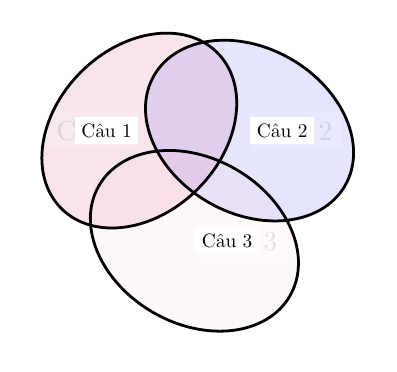
\begin{tikzpicture}[line join = round, line cap = round, line width = 1pt, scale=.7] 
		\coordinate (A) at (0,0);
		\coordinate (B) at (2,0);
			\coordinate (C) at (1,-2);
		\def\goc{45}
		\def\x{1.5}		\def\y{2}
		\draw[rotate=-\goc, fill=purple, opacity=.1] (A) node[left,fill=white]{Câu 1} ellipse (\x cm and \y cm);
		\draw[rotate=-120, fill =blue, opacity=.1] (B) node[right,fill=white]{Câu 2} ellipse (\x cm and \y cm);
			\draw[rotate=-120, fill =pink, opacity=.1] (C) node[right,fill=white]{Câu 3} ellipse (\x cm and \y cm);
		\begin{scope}
			\draw[rotate=-\goc,] (A) node[left,fill=white, scale=.7]{Câu 1}  ellipse (\x cm and \y cm);
			\draw[rotate=-120]  (B)node[right,fill=white, scale=.7]{Câu 2} ellipse (\x cm and \y cm);
			\draw[rotate=-120] (C) node[right,fill=white, scale=.7]{Câu 3} ellipse (\x cm and \y cm);
		\end{scope}
		%\node at ($(A)!.5!(B)$)[fill=white]{\scriptsize $A \cap B$};
	\end{tikzpicture}}
}
\end{bt}
\begin{bt}%[PC06-0-GK1-NH23-24--TeamTeXHoa--Lê Quân]%[0T2K2-2] 
Tìm giá trị lớn nhất  của biểu thức $F(x; y)=x+2y$, biết $\heva{&0\le y\le 4	\\&x\ge 0\\& x-y-1\le 0\\&x+2y-10\le 0.}$
\loigiai{
\immini{
Vẽ các đường thẳng $d_1\colon x-y-1=0$; $d_2\colon x+2y-10=0$ và đường thẳng $d_3\colon y=4$.\\
Miền nghiệm của hệ $\heva{&0\le y\le 4	\\&x\ge 0\\& x-y-1\le 0\\&x+2y-10\le 0}$ là ngũ giác $ABCOE$, trong đó $A(4; 3), B(2; 4), C(0; 4), E(1; 0)$.\\
Ta có $F(4; 3)=10$, $F(2; 4)=10$, $F(0; 4)=8$, $F(1; 0)=1$ và $F(0; 0)=0$.\\
Vậy giá trị lớn nhất của biểu thức $F(x; y)=x+2y$ bằng $10$.}
{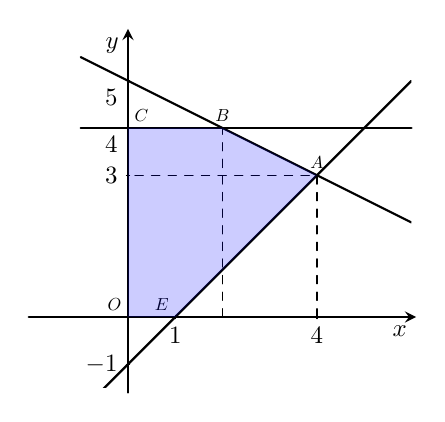
\begin{tikzpicture}[line join=round, line cap=round,>=stealth,thick, scale=.6]
	\tikzset{every node/.style={scale=0.9}}
	\draw[->] (-2.1,0)--(6.1,0) node[below left] {$x$};
	\draw[->] (0,-1.6)--(0,6.1) node[below left] {$y$};
	\draw (0,0) node [above left, scale=.7] {$O$};
	\foreach \x in {1,4}
	\draw[thin] (\x,1pt)--(\x,-1pt) node [below] {$\x$};
	\foreach \y in {-1,3}
	\draw[thin] (1pt,\y)--(-1pt,\y) node [left] {$\y$};
		\draw[thin] (1pt,4)--(-1pt,4) node [below left] {$4$};
		\draw[thin] (1pt,5)--(-1pt,5) node [below left] {$5$};
	\draw[dashed,thin](2,0)--(2,4)--(0,4);
	\draw[dashed,thin](4,0)--(4,3)--(0,3);
	\draw (-1,4)--(6,4);
	\begin{scope}
		\clip (-2,-1.5) rectangle (6,6);
		\draw[samples=200,domain=-1:6,smooth,variable=\x] plot (\x,{(\x)+-1});
		\draw[samples=200,domain=-1:6,smooth,variable=\x] plot (\x,{-0.5*(\x)+5});
	\end{scope}
\draw (1,0) node [above left, scale=.7] {$E$};
\draw (4,3) node [above, scale=.7] {$A$};
\draw (2,4) node [above, scale=.7] {$B$};
\draw (0,4) node [above right, scale=.7] {$C$};
\fill[blue, opacity=.2] (0,0)--(1,0)--(4,3)-- (2,4)--(0,4)--cycle;
\end{tikzpicture}}
}
\end{bt}

\begin{bt}%[PC06-0-GK1-NH23-24--TeamTeXHoa--Lê Quân]%[0T4K2-3] 
Cho tam giác $ABC$ thỏa mãn $\sin A=\dfrac{\sin B+\sin C}{\cos B+\cos C}$. Chứng minh tam giác $ABC$ vuông.
\loigiai{
Ta có \allowdisplaybreaks
\begin{eqnarray*}
\sin A=\dfrac{\sin B+\sin C}{\cos B+\cos C}&\Leftrightarrow& \sin A(\cos B+\cos C)=\sin B+\sin C\\
&\Leftrightarrow& \dfrac{a}{2R}\left(\dfrac{a^2+c^2-b^2}{2ac}+\dfrac{a^2+b^2-c^2}{2ab}\right)=\dfrac{b}{2R}+\dfrac{c}{2R}\\
&\Leftrightarrow& \dfrac{a}{2R}\cdot \dfrac{b(a^2+c^2-b^2)+c(a^2+b^2-c^2)}{2abc}=\dfrac{b+c}{2R}\\
&\Leftrightarrow& b(a^2+c^2-b^2)+c(a^2+b^2-c^2)=2bc(b+c)\\
&\Leftrightarrow& a^2b+bc^2-b^3+a^2c+b^2c-c^3-2b^2c-2bc^2=0\\
&\Leftrightarrow& a^2b-b^3+a^2c-c^3-b^2c-bc^2=0\\
&\Leftrightarrow& (a^2b+ac^2)-(b^3+c^3)-(b^2c+bc^2)=0\\
&\Leftrightarrow& (b+c)(a^2-b^2-c^2)=0\\
&\Leftrightarrow &a^2=b^2+c^2\\
&\Leftrightarrow& \triangle ABC\,\, \text{ vuông tại $A$.} 
\end{eqnarray*}

}
\end{bt}
\Closesolutionfile{ans}
% \inputans{10}{ans/ans-0-GK1-CTST-De8-NH23-24}


